\documentclass[10pt,twocolumn,letterpaper]{article}

\usepackage{cvpr}
\usepackage{times}
\usepackage{epsfig}
\usepackage{graphicx}
\usepackage{amsmath}
\usepackage{amssymb}

% Include other packages here, before hyperref.

% If you comment hyperref and then uncomment it, you should delete
% egpaper.aux before re-running latex.  (Or just hit 'q' on the first latex
% run, let it finish, and you should be clear).
\usepackage[breaklinks=true,bookmarks=false]{hyperref}

\cvprfinalcopy % *** Uncomment this line for the final submission

\def\cvprPaperID{****} % *** Enter the CVPR Paper ID here
\def\httilde{\mbox{\tt\raisebox{-.5ex}{\symbol{126}}}}

% Pages are numbered in submission mode, and unnumbered in camera-ready
%\ifcvprfinal\pagestyle{empty}\fi
\setcounter{page}{1}
\begin{document}

%%%%%%%%% TITLE
\title{Variational Style Transfer}

\author{
Jan Schopohl
% For a paper whose authors are all at the same institution,
% omit the following lines up until the closing ``}''.
% Additional authors and addresses can be added with ``\and'',
% just like the second author.
% To save space, use either the email address or home page, not both
\and
Dominik Fuchsgruber
}

\maketitle
%\thispagestyle{empty}

%%%%%%%%% ABSTRACT
\begin{abstract}
   We propose a variational approach to neural style transfer, where the style of an artistic image is transferred to another. By using variational autoencoders to encode the style of an image, the latent style space is enforced to be smooth. This allows for better interpolation between different styles as well as sampling new unseen styles from the style space.
\end{abstract}

%%%%%%%%% BODY TEXT
\section{Introduction}

The task of artistic style transfer aims to extract the style of an (artistic) image and transfer it to the content of another picture and was first introduced by the seminal work of Gatys et al. in \cite{gatys}. Their approach optimizes a random noise image to fit a particular style and content, which is very demanding computationally-wise. Ever since, many methods were developed that generalize the method proposed in \cite{gatys} to arbitrary styles while also significantly alleviating the computational burden by introducing fully feed-forward neural networks. As has been shown in \cite{adain}, using an encoder-decoder architecture, where the decoder layers are conditioned on a style image using using \textit{Adaptive Instance Normalization} (AdaIn), can achieve visually pleasant results. Instead of using the same encoder module for style and content image, we follow Kotovenko et al. \cite{disentanglement} and make use of distinct encoders for content and style images.

Furthermore, we extend their approach by using a variational autoencoder architecture \cite{vae} to encode the style from an image. This enforces smoothness to the latent style space, which allows for better interpolation between different style embeddings. Furthermore, we are able to draw samples from the latent style space, opening up a generative perspective to our approach.

%-------------------------------------------------------------------------
\section{Related Work}

Artistic style transfer was introduced by Gatys et al. in \cite{gatys}, where the authors noticed, that the style of an image is captured by the gram matrices of different feature maps using the space of a VGG network.   Optimizing a random noise image to minimize the perceptual loss with respect to the content image, while at the same time minimizing the discrepancy of the gram matrices with regards to a style image, leads to a visually appealing stylization. However, their approach suffered from heavy computational requirements, which lead to the development of fully feed-forward architectures for style transfer. \cite{adain} introduces an autoencoder-based approach that is applicable to transfer arbitrary styles the model was not explicitly trained on. They use \textit{Adaptive Instance Normalization}, which manipulates the instance-wise statistics of a content image before each decoder layer, which surprisingly proofed to be sufficient to achieve high quality stylizations. Their method was expanded upon by Kotovenko et al. \cite{disentanglement}, which proposed to incorporate two distinct encoders for content and style images and furthermore introduced a disentanglement loss term that counteracts entanglement of the two latent spaces.

\textit{Adaptive Instance Normalization} is also used to approach different problems, one of which being synthesizing photo-realistic video sequences of speech expressions for a particular individual \cite{talkingheads}. They use AdaIn to condition a decoder module on an embedding of the facial characteristics of a person. In our project, we heavily rely on the architecture of their approach, namely residual blocks both in the encoders and the decoder as well as bottleneck layers between the two. We extend this model by introducing U-Net connections between the content encoder and the decoder module, which was first proposed in \cite{unet}.

The concept of encoding images into a distribution space rather than just embedding them as simple points was first used in \cite{vae}. By sampling from those distributions during training, variations in the latent space can be captured, which leads to a smoother manifold. Furhtermore, the distributions provided by the encoder are regularized to resemble a standard normal, which allows for sampling from the latent space as well.


\section{Our Approach}

We denote with $c \in \mathbb{R}^{3 \times H \times W}$ a content image and analogously with $y \in \mathbb{R}^{3 \times H \times W}$ a style image.

\subsection{Architecture}

Our model consists of three parts: Two distinct encoders for content and style images as well as a decoder that outputs stylizations.
\begin{itemize}
	\item The \textit{content encoder} $E_c$ takes a content image $c$ and applies several convolutions and pooling operations to a content image. It is composed of several residual blocks, and the output still retains a spatial shape, i.e. $E_c(c) \in \mathbb{R}^{D_c \times H^\prime \times W^\prime}$.
	\item The \textit{style encoder} $E_s(s)$ is designed analogously to the content encoder, with the only difference being the use of adaptive pooling after the last convolution. That is, the style encoder yields a fixed-size embedding distribution by outputting the mean and variance of a normal distribution: $E_s(s) \in \mathbb{R}^{2D_s}$.
	\item The \textit{decoder} mirrors the design of the two encoders. It is preceded by several bottleneck layers, which do not change the resolution of the input image. Both the bottleneck layers as well as the upsamling convolutions are conditioned on the style embedding using \textit{Adaptive Instance Normalization}. Additionally, we use U-Net connections that connect the output of content encoder layers to the respective components of the decoder. We denote its output with $y = D(E_c(c), E_s(s))$.
\end{itemize}
	
\begin{figure}
\centering
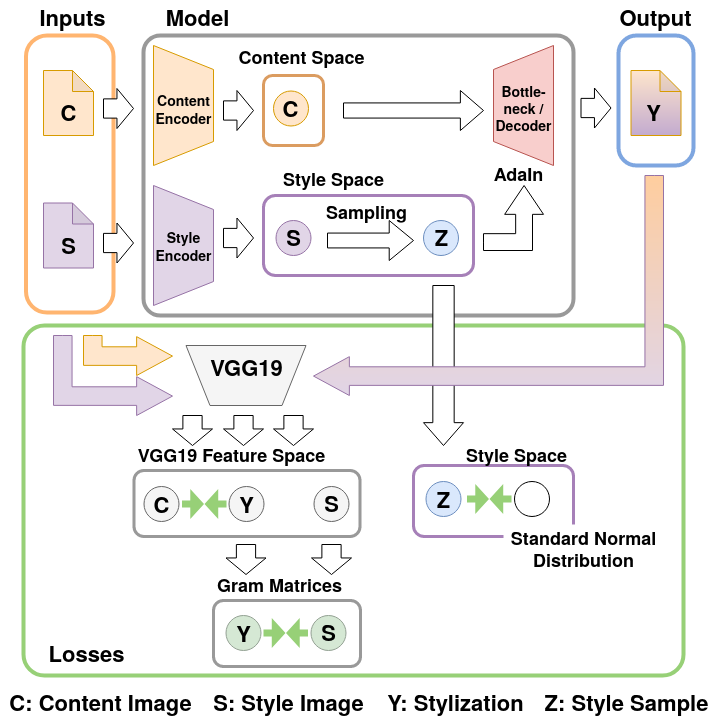
\includegraphics[width=0.9\linewidth]{pipeline_reduced_semi_verbose.png}
\caption{Visualization of the different components in our architecture as well as how the loss terms are implemented. Perceptual and style losses are computed in the VGG19 feature space.}
\label{fig:model}
\end{figure}
	
\subsection{Adaptive Instance Normalization}

Before each convolution in the decoder, the instance wise mean $\mu$ and variance $\sigma^2$ of an image is shifted according to a learnable, linear transformation the style encoding:
\begin{equation}
\{\mu,\sigma^2\} = \mathbf{W}E_s(s) + b
\end{equation}
	
\subsection{Losses}

Our network is trained with respect to three different objectives, two of which are computed in the features space of a pre-trained VGG19 network. Let $VGG^{\{i\}}$ denote the feature maps of the $i$-th layer and $G(x)$ the gram matrix of an activation $x$.
\begin{itemize}
	\item The content loss $\mathcal{L}_{content}$ penalizes deviations of the stylizations regarding the content image and is implemented as a perceptual loss. That is, we consider the feature maps of the $relu_{4,2}$ layer of the VGG19 network.
	\item The style loss $\mathcal{L}_{style}$ penalizes deviations from the style image by comparing the gram matrices of different VGG19 activation maps. We include all layers up to $relu_{4,2}$ into the style loss term.
	\item The variational loss $\mathcal{L}_{KL}$ regularizes the latent space to resemble a standard normal distribution. It uses the Kullback-Leibler divergence to compare the two distributions.
\end{itemize}
\begin{multline}
\mathcal{L}_{content} = \sum_{i} \Vert VGG^{\{i\}}(c) - VGG^{\{i\}}(y)\Vert_2^2 \\
\mathcal{L}_{style} = \sum_{i} \Vert G(VGG^{\{i\}}(c)) - G(VGG^{\{i\}}(y))\Vert_2^2 \\
\mathcal{L}_{KL} = KL(\mathcal{N}(E_s(s)_{:D_s}, E_s(s)_{D_s:}) \Vert \mathcal{N}(0, I))
\end{multline}

We assign different weights $\lambda$ to each component of the content and style loss terms, as well as the variational loss.

\subsection{Datasets}

We use images from the \textit{Places365} dataset \cite{places365}, containing 1.8 million scenic photographs as content images. A subset of 100 images from the \textit{WikiArt} dataset is selected that exhibits a broad range of abstract and artistic styles. We explicitly exclude realistic paintings as they do not contribute to the learning of styles. For both datasets, images are downsampled and cropped to a resolution of $96x96$ pixels.

\section{Results}

\section{Conclusion and Future Work}

{\small
\bibliographystyle{ieee_fullname}
\bibliography{egbib}
}

\end{document}
